% $Header$
\documentclass[xetex]{beamer}
%\usepackage[utf8]{inputenc} % Este paquete permite poner acentos y eñes usando codificación utf-8
\usepackage[spanish]{babel}
\usepackage{listings}
\lstset{language=C,basicstyle=\footnotesize,numbers=left}

\usepackage{xunicode} %Unicode extras!
\usepackage{xltxtra}  %Fixes
\usepackage{fontspec} 
%\fontspec[ItalicFont = OFLGoudyStM-Italic.otf]{OFLGoudyStM.otf}
\setmainfont{OFL Sorts Mill Goudy}
%\setmonofont{OFLGoudyStM.otf}
\setsansfont{OFL Sorts Mill Goudy}
\setromanfont{OFL Sorts Mill Goudy}


%template
\setbeamertemplate{navigation symbols}{} 
\usebackgroundtemplate{
\includegraphics[width=\paperwidth,height=\paperheight]{background}}
\setbeamercolor{alerted text}{fg=white} 
\setbeamercolor{normal text}{fg=white} 
\setbeamercolor{example text}{fg=white} 
\setbeamercolor{structure}{fg=white} 


\title{
\includegraphics[width=6em]{gccegg.pdf}}
\author{Felipe Manzano}
\institute{Machinalis}
\date{16/05/2011}
\subject{Curso en Intel}

\begin{document}

{\usebackgroundtemplate{
\includegraphics[width=\paperwidth,height=\paperheight]{machinalis_a}}
\begin{frame}{}\end{frame}
}

\begin{frame}
  \titlepage
\end{frame}

\begin{frame}
\frametitle{Temas - GCC}
\tableofcontents
\end{frame}

\begin{frame}{}
\section{Introducción}

\begin{quotation}
Compilation refers to the process of converting a program from the
textual source code, in a programming language such as C or C++, into
machine code, the sequence of 1's and 0's used to control the central
processing unit (CPU) of the computer. This machine code is then stored
in a file known as an executable file, sometimes referred to as a binary
file.
\end{quotation}
{\hglue 15em de 'An Introduction to GCC'}
\end{frame}

\begin{frame}{GCC: GNU Compiler Collection}
\begin{itemize}
    \item GNU C Compiler(1987)
    \begin{itemize}
      \item La primer versión de GCC se liberó en 1987
      \item El autor original de este  proyecto es Richard Stallman(el fundador de GNU)
      \item Originalmente, compilaba sólamente C y sus siglas se referían a "GNU C Compiler"
    \end{itemize}

    \item GNU Compiler Collection
    \begin{itemize}
      \item Al 2011 vamos por la versión 4.6.x!
      \item Compila C, C++, Objective-C, Objective-C++, Java, Fortran, y Ada
    \end{itemize}
\end{itemize}
\begin{quotation}
(Vamos a ver solo la parte de C y C++)
\end{quotation}
\end{frame}

\begin{frame}{GCC: Características principales} 
\begin{itemize}
  \item Es portable, anda en cualquier plataforma. Si en Windows también.
  \item Es un cross-compilador; puede compilar código para ser ejecutado en otra plataforma/arquitectura (backends)
  \item Se puede auto-compilar!
  \item Compila diferentes lenguajes (frontends)
  \item Otras: 'fácil' de expandir; es free(GNU)
\end{itemize}  
\end{frame}

\begin{frame}{C y C++ - disclaimer -}
\begin{itemize}
  \item C y C++ son lenguajes de bajo nivel y permiten acceder directamente a la memoria
  \item Hay que prestar mucha atención para no 'tocar' memoria que no se debe tocar
  \item Un bug de corrupción de memoria puede cambiar el comportamiento del programa por completo
  \item GCC tiene algunas heurísticas para detectar algunos de estos errores
  \item Básicamente, usa otro lenguaje
\end{itemize}  
\end{frame}

\section{CC}

\begin{frame}[fragile]{El 'Hola mundo!' en C}
\begin{lstlisting}
#include<stdio.h>
int main (int argc, char *argv[])
{
    printf ("Hola mundo!\n");
}
\end{lstlisting}
%    return 0;

\begin{itemize}
\item Se compila así:
\begin{verbatim}
$gcc holamundo.c -o holamundo
\end{verbatim}
\item La opción \verb=-o= le dice a dónde poner el ejecutable (por defecto: \verb=a.out=)
\item Un editor? \verb=nano/vim/gedit/emacs=
\item tabulado? \verb=indent -i8 holamundo.c=
\end{itemize}

  
\end{frame}
\begin{frame}[fragile]{Prendamos todos los warnings (-Wall)}
  
\begin{itemize}
  \item La opción \verb=-Wall= prende todos los warnings
\begin{verbatim}
holamundo.c: In function 'main':
holamundo.c:4: warning: control reaches end of\
                              non-void function
\end{verbatim}
  \item Los mensajes que genera el GCC siempre tienen la forma:
\begin{verbatim}
file:line-number:message
\end{verbatim}
  \item Ver también \verb=-Wextra= para prender aún más warnings
  \item Con \verb=-Werror= las warnings son consideradas errores
\end{itemize}
\end{frame}

\begin{frame}[fragile]{Compilando desde varios archivos 1/4}
\begin{itemize}
  \item Cualquier programa medianamente serio se divide en módulos/archivos
  \item GCC permite compilar/componer varios archivos de código
\end{itemize}
\begin{lstlisting}
//hello.h:
void hello (const char * name);
\end{lstlisting}

\begin{lstlisting}
hello.c:
#include <stdio.h>
#include "hello.h"
void
hello (const char * name)
{
    printf ("Hello, %s!\n", name);
}
\end{lstlisting}
\end{frame}

\begin{frame}[fragile]{Compilando desde varios archivos 2/4}
\begin{lstlisting}
//main.c:
#include "hello.h"
int
main (void)
{
    hello ("world");
    return 0;
}
\end{lstlisting}

(*) Ver \verb=gcc -E main.c=

\end{frame}

\begin{frame}[fragile]{Compilando desde varios archivos 3/4}
\begin{itemize}
  \item \verb=#include= vs. link, intentando compilar main
\begin{verbatim}
$ gcc -Wall main.c
$ gcc main.c
/tmp/cc4B45wZ.o: In function `main':
main.c:(.text+0x11): undefined reference to `hello'
collect2: ld returned 1 exit status 
\end{verbatim}
  \item Ver salida del preprocesador con:
\begin{verbatim}
$ cpp main.c
\end{verbatim}

  \item O inspeccionar los objetos no definidos con "nm"
\begin{verbatim}
$ gcc main.c -c
$ nm main.o
             U hello
    00000000 T main
\end{verbatim}
\end{itemize}
\end{frame}

\begin{frame}[fragile]{Compilando desde varios archivos 4/4}
\begin{itemize}
  \item Se puede generar un ejecutable directamente de los archivos fuente:
\begin{verbatim}
$gcc -Wall hello.c main.c -o main
\end{verbatim}
  \item Se pueden generar los archivos objeto (.o) por separado:
\begin{verbatim}
$gcc -c -Wall main.c
$gcc -c -Wall hello.c
#generando main.o y hello.o (por defecto)
\end{verbatim}
  \item Y luego "linkear esos dos generando un ejecutable:
\begin{verbatim}
$gcc main.o hello.o -o main
\end{verbatim}
  \item GCC se da cuenta por la extensión del archivo qué debe hacer con él
    (internamente usa: \verb=cpp, cc, g++, ld, ...=)
\end{itemize}
\end{frame}

\begin{frame}[fragile]{Búsqueda de cabeceras (.h)}
\begin{itemize}
  \item Las lineas \verb=#include "FILE.h"= buscan las cabeceras en el directorio actual,
  \item las \verb=#include <FILE.h>= en los configurados en el sistema
  \item Más caminos se pueden agregar con \verb=-I=: \verb=gcc -I /misheaders/ -Wall hello.c main.c -o main=
  \item y además se pueden pasar varias veces: 
  \begin{verbatim}
gcc -I /misheaders1/ -I /misheaders2/ code.c
\end{verbatim}
    \item La variable de entorno \verb=C_INCLUDE_PATH= contiene más directorios donde buscar
\end{itemize}
\end{frame}

\begin{frame}[fragile]{Bibliotecas y signaturas por defecto (1/4)}

\begin{lstlisting}
/*printflt.c*/
#include<stdio.h>
void printflt (float f){
    printf("%f\n",f);
}
/*printflt.h*/
void printflt (float f);
\end{lstlisting}
\begin{itemize}

  \item Generamos una biblioteca libpflt.a con esta función:
\begin{verbatim}
$gcc -c printflt.c
$ar rvs libpflt.a printflt.o
\end{verbatim}
\end{itemize}
\end{frame}

\begin{frame}[fragile]{Bibliotecas y signaturas por defecto (2/4)}
  
\begin{lstlisting}
/* main.c: */
/*#include "printflt.h"*/
int main (void){
    printflt (0.12345);
    return 0;
}
\end{lstlisting}
\begin{itemize}
  \item Esto se compila así: \verb=gcc -Wall main.c -lpflt -L./ -o main=
\end{itemize}
\end{frame}

\begin{frame}[fragile]{Búsqueda de bibliotecas y signaturas por defecto (3/4)}
  

\begin{itemize}
  \item Como no incluimos la cabecera printflt.h donde está declarada 'prinflt', GCC usa
una signatura por defecto que es incompatible, en algunas arquitecturas
ésto es catastrófico para cierta combinacion de tipos
  \item Sin embargo GCC nos avisa de esto con un warning:
\begin{verbatim}
gcc -Wall main.c -o main
main.c: In function 'main':
main.c:3: warning: implicit declaration of\
                        function 'printflt'
\end{verbatim}

\end{itemize}
  
\end{frame}
\begin{frame}[fragile]{Búsqueda de bibliotecas y signaturas por defecto (4/4)}
\begin{itemize}
\item La biblioteca con la definición de \verb=printflt= es \verb=libprintflt.a= 
\item Generalmente las bibliotecas instaladas en el sistema se encuentran en: \verb=/lib=, y \verb=/usr/lib=
\item Para linkear con \verb=libprintflt.a= se agrega el parámetro \verb=-lprintflt= (GCC buscará \verb=libprintflt.a=)
\item La opción \verb=-lNAME= intenta enlazar los archivos objeto con la biblioteca \verb=‘libNAME.a’= que debe estar en los directorios estándard
\item Más directorios de búsqueda de bibliotecas de pueden agregar con \verb=-L= o con la variable de entorno \verb=LIBRARY_PATH=
\end{itemize}
\end{frame}

\begin{frame}[fragile]{Directorios donde buscar cabeceras y bibliotecas.}
\begin{itemize}
  \item En resumen, GCC busca las cabeceras y bibliotecas:
  \begin{itemize}
    \item en los directorios pasados con \verb=-I= y \verb=-L=
    \item o en las variables de entorno:
\begin{verbatim}
C_INCLUDE_PATH=path1:path2:path3
LIBRARY_PATH=path1:path2:path3
\end{verbatim}
  \item y por último en las preconfiguradas en gcc (ver gcc -v)
            (/usr/include/, /usr/lib/, /lib/)
  \end{itemize}
\end{itemize}
\end{frame}

\begin{frame}[fragile]{El preprocesador - ejemplito }
  

\begin{lstlisting}
/* test.c: */
#include <stdio.h>
int main (void) {
#ifdef TEST
    printf ("Test mode\n");
#endif
    printf ("Running...\n");
    return 0;
}
\end{lstlisting}
\end{frame}

\begin{frame}[fragile]{El preprocesador}
\begin{itemize}
  \item El preprocesador ejecuta antes que la compilación cambiando posiblemente el
    programa
  \item Las 'variables' de pre-procesamiento se pueden definir:
\begin{itemize}
  \item con \verb=#define= desde cualquier parte del código:
\verb=#define TEST 1=
  \item o desde la línea de comando con \verb=-D= p.ej.
\verb#gcc -DTEST=1 test.c -o test#
\end{itemize}
  \item Para investigar el código después del pre procesamiento hacer:
\begin{verbatim}
gcc -E -DTEST test.c
gcc -E test.c
\end{verbatim}
\end{itemize}
\end{frame}


\begin{frame}[fragile]{Compilar para depuración}

\begin{itemize}
  \item Esto introduce meta-datos de depuración en el ejecutable
\verb=gcc -ggdb -o test test.c=
  \item Para mantener una copia de la información de depuración
\verb=cp test test.debug=
\verb=strip --only-keep-debug test.debug=
  \item Para borrar esta información antes de un release se puede hacer:
strip test
  \item Para volver a introducir la info de debug:
\verb#objcopy --add-gnu-debuglink=test.debug test#
  \item Cuidado con las optimizaciones. Ej: \verb=-fomit-frame-pointer= y \verb=-O4=
\end{itemize}
\end{frame}

\section{Optimizaciones}

\begin{frame}[fragile]{Optimizaciones}
\begin{itemize}
  \item Las optimizaciones se controlan principalmente con el parámetro \verb=-Ox= (\verb=0,1,2,3,s=)
  \item Otro parámetro interesante es \verb=-funroll-loops=
  \item Desde el código mismo se pueden usar funciones inline y variables en registros
  \item También se pueden usar fragmentos de assembler...
\begin{verbatim}
int x,n;
asm ("popcnt %1, %0"
      : "=r" (n) /*outputs*/
      : "r" (x)  /*inputs*/
      /*no clobbered*/
      );
\end{verbatim}
  \item \verb=gcc -s file.c genera file.s=
\end{itemize}

  
\end{frame}
\begin{frame}[fragile]{Probamos esto con diferentes optimizaciones..}
  
\begin{lstlisting}
#include <stdio.h>
double powern (double d, unsigned n) {
    double x = 1.0;
    unsigned j;
    for (j = 1; j <= n; j++)
       x *= d;
    return x;
}
int main (void) {
    double sum = 0.0;
    unsigned i;
    for (i = 1; i <= 100000000; i++) {
        sum += powern (i, i % 5);
    }
    printf ("sum = %g\n", sum);
    return 0;
}
\end{lstlisting} 
\end{frame}
\begin{frame}[fragile]{Comparativas de las optimizaciones}
  

\begin{verbatim}

gcc -Os test.c -o test                  0m6.738s ?
gcc -O0 test.c -o test                  0m6.413s
gcc -O1 test.c -o test                  0m4.114s
gcc -O2 test.c -o test                  0m3.200s
gcc -O3 test.c -o test                  0m3.196s
gcc -O3  -funroll-loops test.c -o test  0m2.856s
clang(llvm2.8)                          0m2.635s
(Intel(R) Core(TM)2 CPU         T5500  @ 1.66GHz)
\end{verbatim}

  
\end{frame}

\section{G++}


\begin{frame}[fragile]{Hola mundo en C++ (1/2)}
  
\begin{lstlisting}
include <iostream>
int main ()
{
    std::cout << "Hola c++!" << std::endl;
    return 0;
}
\end{lstlisting}

\begin{itemize}
  \item Se compila así:
\begin{verbatim}
$ g++ holamundo.cc -o holamundocc
$ holamundocc
Hola c++!
\end{verbatim}
\end{itemize}

\end{frame}

\begin{frame}[fragile]{Hola mundo en C++ (2/2)}
\begin{itemize}
  \item Generalmente se usa \verb=.cc=, \verb=.cpp=, \verb=.cxx= o \verb=.C=
  \item \verb=GCC= provee el compilador de c++ 'g++'
  \item Ambos compiladores comparten muchos de los parámetros
  \item Los programas en \verb=C++= DEBEN enlazarse usando \verb=g++= para que se utilicen las bibliotecas apropiadas
  \item Las bibliotecas de C++ son parte de GCC
\end{itemize}  
\end{frame}

\begin{frame}[fragile]{Templates 1/3 - libstdc++}
\begin{itemize}
  \item Los templates se consideran una especie de *super* macro
  \item Cuando una clase con template se usa con determinado tipo de datos, la 'plantilla' correspondiente se compila con este tipo de dato sustituido donde corresponde
  \item Los templates estándar como \verb='list'= se usan directamente
\end{itemize}
\begin{lstlisting}
/* lists.c: */
#include <list>
#include <string>
#include <iostream>
using namespace std;
int main () {
    list<string> list;
    list.push_back("Hello");
    list.push_back("World");
    cout << "List size = " << list.size() << endl;
    return 0;
}

//g++ -Wall string.cc
\end{lstlisting}
\end{frame}

\begin{frame}[fragile]{Templates 2/3 - Mis templates}
\begin{itemize}
  \item Se pueden definir templates a gusto
  \item Se recomienda incluir tanto la declaración como la definición de las clases
con templates en la cabecera ( inclusion compilation model)
  \item Se usan macros del pre-procesador para evitar que la clase se parsee varias veces
  \item \verb=g++= compila la definición apropiada de la clase del \verb=.h= en el momento en que es usada
  \item La versión compilada de la clase se pone en el archivo objeto (\verb=.o=)
  \item Funciona sólo con el GNU Linker
\end{itemize}
\end{frame}

\begin{frame}[fragile]{Templates 3/3 - aha, pero no quiero poner todo en el {\tt .h}}  
\begin{itemize}
  \item Instanciación EXPLÍCITA de templates: \verb=-fno-implicit-templates=
  \item Las funciones 'templatizadas' no se compilan en el punto en el que son usadas
  \item \verb=g++= busca los keywords \verb=template ClassName<type>= y fuerza la compilación de la versión del template especificada
  \item Si se hace bien esto asegura que la compilación de cierto template para
cierto tipo aparezca sólo una vez en los archivos objeto (\verb=.o=)
  \item Contra: es necesario saber de antemano qué instanciaciones se van a necesitar
\end{itemize}
\end{frame}

\section{Funcionamiento interno GCC}

\begin{frame}[fragile]{Funcionamiento interno del GCC (1/2)}
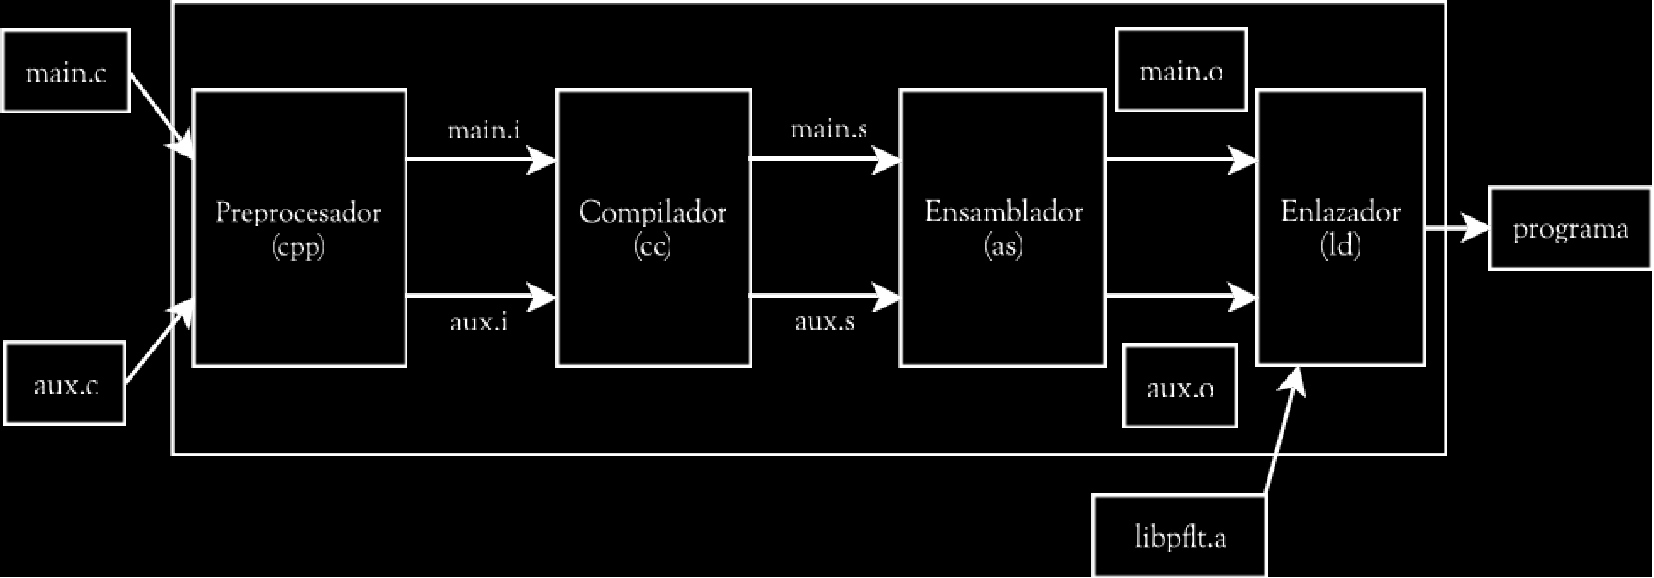
\includegraphics[width=\textwidth]{compilation_stagesI.pdf}
\begin{itemize}
  \item GCC pasa por las siguientes etapas:
\begin{enumerate}
  \item Pre procesamiento: expande las macros (\verb=gcc -E=)
  \item Compilación: de código fuente a assembler (\verb=gcc -S=)
  \item Ensamblado: de assembler a código máquina (\verb=as=)
  \item Enlazado: arma el ejecutable a partir de los archivos objeto (\verb=ld=)
\end{enumerate}
\end{itemize}
\end{frame}

\begin{frame}[fragile]{Funcionamiento interno del GCC (2/2)}
  
\begin{lstlisting}
#include <stdio.h>
int
main (void)
{
    printf ("Hello, mundo!\n");
    return 0;
}
\end{lstlisting}

\begin{itemize}
  \item \verb=cpp holamundo.c -o holamundo.i    #(gcc -E)=
  \item \verb=gcc -S holamundo.i -o holamundo.s #(gcc -S)=  
  \item \verb=as holamundo.s -o holamundo.o     #(gcc -c)=
  \item \verb=ld holamundo.o ???????? -o holamundo.exe=
(Hay que incluir muchas bibliotecas estandar y de inicialización ver \verb=gcc -v holamundo.o=)
\end{itemize}
  
\end{frame}

\begin{frame}[fragile]{Opciones específicas de la plataforma}
\begin{itemize}
  \item Son las opciones que empiezan con \verb=-m=
  \item \verb#-march=xxx# decide el procesador destino (\verb=native=, \verb=athlon=, \verb=core2=)
  \item \verb#-mtune=xxx# selecciona sólo el ordenamiento(scheduling) de instrucciones
  \item Cada procesador tiene su conjunto de opciones p.ej en Intel et.al. :
\begin{itemize}
  \item \verb=-m32= compila para 32 bits en hosts de 64
  \item \verb=-msse4= habilita el uso de instrucciones específicas
\end{itemize}
  \item Ejemplo optimize.c específico para mi máquina:
\begin{verbatim}
$ gcc -march=native -O3 optimize.c -funroll-loops 
                      -o optimizeGCCO3UnrollCore2
$ time ./optimizeGCCO3UnrollCore2  0m1.168s !!
\end{verbatim}
\end{itemize}
\end{frame}

\section{Seguridad}


\begin{frame}[fragile]{Seguridad 1/2 - Anti stack overflow}
\begin{itemize}
  \item La opción \verb=-fstack-protector= agrega protección contra ataques por
desbordamientos de la pila (también \verb=-fstack-protector-all=)
\begin{itemize}
  \item El código binario queda un poco mas grande y lento
  \item A cada función pertinente se le agrega un prólogo y epílogo
  \item Al principio de la función se apila un valor local implicito y 'aleatorio'
  \item A la salida se revisa que este valor siga siendo el mismo que al inicio
  \item Este simple check previene una importante gama de ataques
  \item Y sirve para depurar más fácilmente esta clase de errores
\end{itemize}
\end{itemize}
\begin{verbatim}
overflow.c:
    memset(alloca(1),'A',1000);
\end{verbatim}
  
\end{frame}
\begin{frame}[fragile]{Seguridad 2/2 - Anti format string bug}
\begin{itemize}
  \item Se da cuando una format string es controlada por el entorno
  \item En Linux toda la familia de funciones de printf/syslog/scanf están afectadas
  \item Estos son los parámetros de GCC relacionados :
     \begin{itemize}
        \item \verb#-Wformat#, 
        \item \verb#-Wno-format-extra-args#,
        \item \verb#-Wformat-security#, 
        \item \verb#-Wformat-nonliteral#, 
        \item \verb#-Wformat=2#
     \end{itemize}
\end{itemize}
\begin{verbatim}
formatstr.c:
    printf("%n%n%n%n%n%n%n%n%n%n%n%n%n%n");
\end{verbatim}
\end{frame}

\section{Instrumentación}

\begin{frame}[fragile]{Misc 1/2 GNU Profiler (gprof)}
\begin{itemize}
  \item \verb=gcc -pg test.c -o test= genera un binario instrumentado
  \item Una ejecución del ejecutable resultante genera un archivo \verb=gmon.out=
  \item \verb=gmon.out= guarda la información necesaria para contar cuánto tiempo se utilizó en cada función del programa
  \item Util para seleccionar qué función mejorar
  \item Se prueba así:
\begin{verbatim}
gcc -pg test.c -o test #binario instrumentado
./test       #genera el gmon.out silenciosamente
gprof test   #muestra los datos recopilados
\end{verbatim}
\end{itemize}
\end{frame}

\begin{frame}[fragile]{Misc 2/2 GNU Coverage (gcov)}
  
\begin{itemize}
  \item Es una herramienta de testing que cuenta cuantas veces se pasa por
    cierta línea en una ejecución del programa
  \item De esta manera se podría ver qué partes del programa han sido testeadas o no
  \item Se usa así:
\begin{verbatim}
gcc -fprofile-arcs -ftest-coverage test.c -o test
./test      #recopila datos de la traza de ejecución
gcov test  #genera un archivo test.gcov
\end{verbatim}
  \item Los archivos \verb=.gcov= generados son una copia del código fuente con un
    número indicando cuántas veces se ha pasado por esa línea
\end{itemize}
\end{frame}

\section{Extensiones de GCC}

\begin{frame}[fragile]{Extensiones de gcc 1/3 - Inicializadores}

Ref. \url{http://gcc.gnu.org/onlinedocs/gcc/C-Extensions.html}
\begin{itemize}
  \item En ISO C99 esto:
\begin{lstlisting}
int a[6] = { [4] = 29, [2] = 15 };
\end{lstlisting}
    es lo mismo que hacer:
\begin{lstlisting}
int a[6] = { 0, 0, 15, 0, 29, 0 };
\end{lstlisting}

  \item GCC permite otras macumbas:
\begin{lstlisting}
int widths[] = { [0 ... 9] = 1, 
                 [10 ... 99] = 2,  
                 [100] = 3 };
\end{lstlisting}

\end{itemize}
  
\end{frame}

\begin{frame}[fragile]{Extensiones de gcc 2/3 - Arreglos de longitud zero}
  
\begin{lstlisting}
/* arrayzero.c: */
struct line {
 int length;
 char contents[0];
};
struct line * new_line(char* str){
  this_length = strlen(str);
  struct line *thisline = (struct line *)
    malloc (sizeof (struct line) + this_length);
  thisline->length = this_length;
  strcpy(thisline->contents,str);
  return thisline;
}
\end{lstlisting}

\verb=$gcc -Wall arrayzero.c -o arrayzero=

\end{frame}

\begin{frame}[fragile]{Extensiones de gcc 3/3 - Arreglos de longitud variable}
  
\begin{lstlisting}
/* bopen2.c: */
int
open2 (char *str1, char *str2, int flags, int mode)
{
  char name[strlen(str1) + strlen(str2) + 1];
  stpcpy (stpcpy (name, str1), str2);
  return open (name, flags, mode);
}
/*
opcion:
char *name = (char *) 
        alloca (strlen(str1) + strlen(str2) + 1);
*/
\end{lstlisting}  
\end{frame}
\section{Crosscompilación}
\begin{frame}{Crosscompilación}
\begin{itemize}
  \item Método para generar ejecutables en una arquitectura y SO (host) para
    ser usado en otra arquitectura y/o sistema hiperactivo (target)
  \item Se necesita una toolchain específica para cada combinación host/target
  \item Compilador que genere el assembler apropiado
  \item Ensamblador que genere binarios apropiados
  \item Linker que pueda generar ejecutables del tipo apropiados
  \item Bibliotecas estándares compiladas para el target específico (syscalls?)
  \item Existen conjuros para generar estas toolchains (ver crosstool de Dan Kegel)
  \item Otras toolchains para targets populares se pueden bajar directamente (android)
\end{itemize}
\end{frame}

\begin{frame}
 \frametitle{Crosscompilación - Hands on}
\begin{quotation}
A cross compiler is a compiler capable of creating
executable code for a platform other than the one
on which the compiler is run.
\end{quotation}

\begin{itemize}
  \item Esto se vuelve aún más interesante cuando el target es embedded
  \item Otro motivo: compilación distribuida
\end{itemize}
\end{frame}

\begin{frame}{Crosscompilación - El toolchain}

\begin{itemize}
\item Necesitamos un compilador, un ensamblador, un enlazador y las bibliotecas que ejecutarán en el destino; es decir un toolchain
\item Varios scripts que automatizan la creacion de esto:
\begin{itemize}
  \item Dan Kegel - http://www.kegel.com/crosstool/
  \item Gentoo Cross - toolchain generator - emerge crossdev
  \item crosstool-ng - http://crosstool-ng.org/download/crosstool-ng
\end{itemize}
\end{itemize}
\end{frame}

\begin{frame}[fragile]{Crosscompilación - crosstool-ng}
\begin{verbatim}
$ mkdir ~/crosstool-ng
$ cd ~/crosstool-ng
$ wget http://crosstool-ng.org/download/crosstool-ng/
                          crosstool-ng-1.11.1.tar.bz2
$ sha1sum  crosstool-ng-1.11.1.tar.bz2 
7d992265fc77c19331da0d61b0c8fb58209f4998 
\end{verbatim}
\end{frame}

\begin{frame}[fragile]{Crosscompilación - crosstool-ng}
\begin{verbatim}
$ tar jxvf crosstool-ng-1.11.1.tar.bz2
$ cd crosstool-ng-1.11.1
$#sudo zypper install make gcc bison flex texinfo libtool
$#      cvs patch lzma ncurses-devel gcc-c++ glibc-static
$ ./configure --prefix=/opt/crosstool-ng
$ make
$ sudo make install
\end{verbatim}
\end{frame}

\begin{frame}[fragile]{Crosscompilación - Configuración de la toolchain}
\begin{itemize}
  \item Copiar \verb=PENDRIVE/src= a \verb=$HOME= para que no baje todos denuevo
  \item Preparar un directorio de trabajo
\begin{verbatim}
$ mkdir -p ~/crosstool-ng/crosstool-ng-build
$ cd ~/crosstool-ng/crosstool-ng-build
\end{verbatim}
  \item Revisar los ejemplos pre-configurados y elegir uno
\begin{verbatim}
$ ls /opt/crosstool-ng/lib/ct-ng-1.11.1/samples/
$ cp /opt/crosstool-ng/lib/ct-ng-1.11.1/samples/
               arm-unknown-linux-uclibcgnueabi/* .
$ mv crosstool.config .config
\end{verbatim}
\item Debe quedar un \verb=.config= y su \verb=uClibc.config= asociado en el directorio de trabajo (failsafe usar \verb=.config= y \verb=uClibc.config= provisto en el pendrive)

  \item Configurar, bajar y construir la toolchain
\begin{verbatim}
$ export PATH=/opt/crosstool-ng/bin:$PATH
$ ct-ng menuconfig
$ ct-ng build.4
\end{verbatim}

\end{itemize}
\end{frame}

\begin{frame}[fragile]{Crosscompilación - Hola mundo para ARM}
  
\begin{lstlisting}
/* armholamundo.c: */
int main(void){
    printf("Hola, ARM!\n");
return 0;
}
\end{lstlisting}  
\begin{verbatim}
$ ~/x-tools/arm-unknown-linux-uclibcgnueabi/bin/\
arm-unknown-linux-uclibcgnueabi-gcc -static holamundo.c\ 
                                        -o holamundo.arm
$ adb -e push holamundo.arm /data/holamundo.arm
$ adb -e shell
# cd data	
# chmod +755 holamundo.arm
# ./holamundo.arm
Hola, ARM! 
\end{verbatim}
\end{frame}


\section{Compilación distribuida}

\begin{frame}{distcc: Compilación distribuida}
\begin{itemize}
  \item distcc ditribuye la compilación de proyectos grandes en varias 
        computadoras en red
  \item Soporta C y C++
  \item Genera los mismos resultados que una compilación local
  \item Fácil de instalar y a veces más rápido que compilar todo local
  \item Las diferentes máquinas sólo necesitan tener un compilador apropiado
  \item Ref. \url{http://code.google.com/p/distcc/}
\end{itemize}
\end{frame}

\begin{frame}[fragile]{distcc: Compilación distribuida 2/3}
\begin{verbatim}
$ wget http://distcc.googlecode.com/files/\
                         distcc-3.1.tar.bz2
$ sha1sum distcc-3.1.tar.bz2
$30663e8ff94f13c0553fbfb928adba91814e1b3a 
$ tar jxvf distcc-3.1.tar.bz2
$ cd distcc-3.1
$ ./configure
$ make
$ sudo make install
\end{verbatim}
\end{frame}

\begin{frame}[fragile]{distcc: Compilación distribuida 3/3}
\begin{itemize}
\item Otra: \verb=sudo yum install distcc =
\item Lo importante es que el server alcance el gcc apropiado
\item Manualmente el server se usa así: 
\begin{verbatim}
$ export PATH=~/x-tool/ ... .../bin:$PATH
$ gcc -v 
$ distccd --daemon --allow 192.168.1.0/24
\end{verbatim}
\item y el cliente así:
\begin{verbatim}
$ export DISTCC_HOSTS="192.168.1.101 192.168.1.102"
$ CC=distcc
$ distcc -static holamundo.c -o holamundo
\end{verbatim}
\end{itemize}
\end{frame}

\begin{frame}[fragile]{Cross-compilación distribuida!}
\begin{verbatim}
cd ~/x-tools/ ... /bin
for file in *; do
    ln -s $file ${file#arm-unknown-linux-uclibcgnueabi-}
done
$ gcc -v
$ distccd --allow 192.168.1.0/24
\end{verbatim}
Sacado de \url{http://plugapps.com/index.php5/Developers:_Cross-Compiling_with_distcc}
\end{frame}


\begin{frame}[fragile]{distcc: Compilación distribuida de joe 1/2}
\begin{verbatim}
$ wget http://downloads.sourceforge.net/project/\
   joe-editor/JOE\ sources/joe-3.7/joe-3.7.tar.gz  
$ sha1sum joe-3.7.tar.gz 
54398578886d4a3d325aece52c308a939d31101d 
$ tar xvf joe-3.7.tar.gz
$ cd joe-3.7
$ chmod +x configure
$ ./configure --prefix=/system/local \
--disable-curses --disable-termcap --disable-termidx \ 
CFLAGS=" -static $_XXFLAGS" ARCH=arm \
--host=arm-unknown-linux-uclibcgnueabi \
CC="arm-unknown-linux-uclibcgnueabi-gcc" \ 
CROSS_COMPILE="arm-unknown-linux-uclibcgnueabi-" \ 
sysconfdir=/system/usr/local/etc sysconfjoesubdir=/joe 
\end{verbatim}
{\small Sacado de \url{http://www.curtisembedded.com/wiki/bin/view/Android/CrosstoolsAndBuilding}}
\end{frame}



\begin{frame}[fragile]{distcc: Compilación distribuida de joe 2/2}
\begin{verbatim}

$ export DISTCC_HOSTS="127.0.0.1 192.168.1.106"
$ export DISTCC_VERBOSE=1
$ time pump make -j8 CC=distcc
..
$ adb -e push joe /data/joe
$ adb -e shell
# cd data
# chmod 755 joe
# TERM=ansi ./joe archivo.txt
 
\end{verbatim}
\end{frame}



\section{Referencias}

\begin{frame}[fragile]{Referencias}
\begin{itemize}
\item \url{http://gcc.gnu.org/}
\item \url{www.karunya.edu/linuxclub/resources/GCC.pdf}
\item \verb=info gcc=
\item \url{http://crosstool-ng.org/hg/crosstool-ng/file/tip/docs/}
\item \url{http://code.google.com/p/distcc/}
\item \url{mailto:felipe.andres.manzano@gmail.com}
\end{itemize}
\end{frame}
 
{\usebackgroundtemplate{
\includegraphics[width=\paperwidth,height=\paperheight]{machinalis_b}}
\begin{frame}{}\end{frame}
}

\end{document}

